% Template of basic phisics experiment 基于 article template,在此基础上做修改
% 设定文章编码类型,正文字号为五号则 zihao=5,正文字号为小四则 zihao=-4
\documentclass[zihao=5, UTF8]{article}		


% 自定义宏定义
\def\N{\mathbb{N}}
\def\F{\mathbb{F}}
\def\Z{\mathbb{Z}}
\def\Q{\mathbb{Q}}
\def\R{\mathbb{R}}
\def\C{\mathbb{C}}
\def\T{\mathbb{T}}
\def\S{\mathbb{S}}
\def\A{\mathbb{A}}
\def\I{\mathscr{I}}
\def\d{\mathrm{d}}
\def\p{\partial}


% 物理实验报告所需的其它宏包
\usepackage{ulem}   % \uline 下划线支持

% 导入基本宏包
\usepackage[UTF8]{ctex}     % 设置文档为中文语言
\usepackage[colorlinks, linkcolor=blue, anchorcolor=blue, citecolor=blue, urlcolor=blue]{hyperref}  % 宏包:自动生成超链接 (此宏包与标题中的数学环境冲突)
% \usepackage{docmute}    % 宏包:子文件导入时自动去除导言区,用于主/子文件的写作方式,\include{./51单片机笔记}即可。注:启用此宏包会导致.tex文件capacity受限。
\usepackage{amsmath}    % 宏包:数学公式
\usepackage{mathrsfs}   % 宏包:提供更多数学符号
\usepackage{amssymb}    % 宏包:提供更多数学符号
\usepackage{pifont}     % 宏包:提供了特殊符号和字体
\usepackage{extarrows}  % 宏包:更多箭头符号

% 列表环境设置
\usepackage{enumitem}   % 宏包:列表环境设置
    \setlist[enumerate]{itemsep=0pt, parsep=0pt, topsep=0pt, partopsep=0pt, leftmargin=3.5em} 
    \setlist[itemize]{itemsep=0pt, parsep=0pt, topsep=0pt, partopsep=0pt, leftmargin=3.5em}
    \newlist{circledenum}{enumerate}{1} % 创建一个新的枚举环境  
    \setlist[circledenum,1]{  
        label=\protect\circled{\arabic*}, % 使用 \arabic* 来获取当前枚举计数器的值,并用 \circled 包装它  
        ref=\arabic*, % 如果需要引用列表项,这将决定引用格式(这里仍然使用数字)
        itemsep=0pt, parsep=0pt, topsep=0pt, partopsep=0pt, leftmargin=3.5em
    }  
% 文章页面 margin 设置
\usepackage[a4paper]{geometry}  % 宏包:文章页面 margin 设置
    \geometry{top=0.75in}
    \geometry{bottom=0.75in}
    \geometry{left=0.75in}
    \geometry{right=0.75in}   % 设置上下左右页边距
    \geometry{marginparwidth=1.75cm}    % 设置边注距离(注释、标记等)

% 自定义数学环境
\usepackage{amsthm} % 宏包:数学环境配置
% theorem-line 环境自定义
    \newtheoremstyle{MyLineTheoremStyle}% <name>
        {11pt}% <space above>
        {11pt}% <space below>
        {}% <body font> 使用默认正文字体
        {}% <indent amount>
        {\bfseries}% <theorem head font> 设置标题项为加粗
        {:}% <punctuation after theorem head>
        {.5em}% <space after theorem head>
        {\textbf{#1}\thmnumber{#2}\ \ (\,\textbf{#3}\,)}% 设置标题内容顺序
    \theoremstyle{MyLineTheoremStyle} % 应用自定义的定理样式
    \newtheorem{LineTheorem}{Theorem.\,}
% theorem-block 环境自定义
    \newtheoremstyle{MyBlockTheoremStyle}% <name>
        {11pt}% <space above>
        {11pt}% <space below>
        {}% <body font> 使用默认正文字体
        {}% <indent amount>
        {\bfseries}% <theorem head font> 设置标题项为加粗
        {:\\ \indent}% <punctuation after theorem head>
        {.5em}% <space after theorem head>
        {\textbf{#1}\thmnumber{#2}\ \ (\,\textbf{#3}\,)}% 设置标题内容顺序
    \theoremstyle{MyBlockTheoremStyle} % 应用自定义的定理样式
    \newtheorem{BlockTheorem}[LineTheorem]{Theorem.\,} % 使用 LineTheorem 的计数器
% definition 环境自定义
    \newtheoremstyle{MySubsubsectionStyle}% <name>
        {11pt}% <space above>
        {11pt}% <space below>
        {}% <body font> 使用默认正文字体
        {}% <indent amount>
        {\bfseries}% <theorem head font> 设置标题项为加粗
        {:\\ \indent}% <punctuation after theorem head>
        {0pt}% <space after theorem head>
        {\textbf{#3}}% 设置标题内容顺序
    \theoremstyle{MySubsubsectionStyle} % 应用自定义的定理样式
    \newtheorem{definition}{}


% 有色文本框及其设置
\usepackage[dvipsnames,svgnames]{xcolor}    %设置插入的文本框颜色
\usepackage[strict]{changepage}     % 提供一个 adjustwidth 环境
\usepackage{framed}     % 实现方框效果
    \definecolor{graybox_color}{rgb}{0.95,0.95,0.96} % 文本框颜色。修改此行中的 rgb 数值即可改变方框纹颜色,具体颜色的rgb数值可以在网站https://colordrop.io/ 中获得。(截止目前的尝试还没有成功过,感觉单位不一样)(找到喜欢的颜色,点击下方的小眼睛,找到rgb值,复制修改即可)
    \newenvironment{graybox}{%
    \def\FrameCommand{%
    \hspace{1pt}%
    {\color{gray}\small \vrule width 2pt}%
    {\color{graybox_color}\vrule width 4pt}%
    \colorbox{graybox_color}%
    }%
    \MakeFramed{\advance\hsize-\width\FrameRestore}%
    \noindent\hspace{-4.55pt}% disable indenting first paragraph
    \begin{adjustwidth}{}{7pt}%
    \vspace{2pt}\vspace{2pt}%
    }
    {%
    \vspace{2pt}\end{adjustwidth}\endMakeFramed%
    }

% 各级标题自定义设置
\usepackage{titlesec}   
    % section标题自定义设置 
    \titleformat{\section}[hang]{\normalfont\huge\bfseries\centering}{第\,\thesection\,部分}{20pt}{}
    % subsection标题自定义设置 
    \titleformat{\subsection}[hang]{\normalfont\Large\bfseries}{\,\thesubsection\,}{8pt}{}
    % subsubsection标题自定义设置
    \titleformat{\subsubsection}[hang]{\normalfont\large\bfseries}{\,\thesubsubsection\,}{6pt}{}

% 外源代码插入设置
\usepackage{matlab-prettifier}
    \lstset{
        style=Matlab-editor,  % 继承matlab代码颜色等
    }
\usepackage[most]{tcolorbox} % 引入tcolorbox包 
\usepackage{listings} % 引入listings包
    \tcbuselibrary{listings, skins, breakable}
    \lstdefinestyle{matlabstyle}{
        language=Matlab,
        basicstyle=\small,
        breakatwhitespace=false,
        breaklines=true,
        captionpos=b,
        keepspaces=true,
        numbers=left,
        numbersep=15pt,
        showspaces=false,
        showstringspaces=false,
        showtabs=false,
        tabsize=2
    }
    \newtcblisting{matlablisting}{
        arc=0pt,
        top=0pt,
        bottom=0pt,
        left=1mm,
        listing only,
        listing style=matlabstyle,
        breakable,
        colback=white   % 选一个合适的颜色
    }
    % 自定义Verilog代码样式
\lstdefinelanguage{Verilog}{
    keywords=[1]{module, input, output, wire, assign, endmodule},
    keywords=[2]{always, if, else, case, endcase, begin, end},
    sensitive=true,
    morecomment=[l]{//},
    morecomment=[s]{/*}{*/},
    morestring=[b]",
}

\lstset{
    language=Verilog,
    basicstyle=\ttfamily\small,
    keywordstyle=[1]\color{blue},
    keywordstyle=[2]\color{purple},
    commentstyle=\color{gray},
    stringstyle=\color{orange},
    showstringspaces=false,
    numbers=left,
    numberstyle=\tiny\color{gray},
    stepnumber=1,
    numbersep=5pt,
    frame=single,
    tabsize=4,
    breaklines=true,
    backgroundcolor=\color{lightgray!10}
}

% table 支持
\usepackage{booktabs}   % 宏包:三线表
\usepackage{tabularray} % 宏包:表格排版
\usepackage{longtable}  % 宏包:长表格
\usepackage{tabularx}  % 宏包:宽表格
\usepackage{multirow}  % 宏包:表格中一格显示多个项目

% figure 设置
\usepackage{graphicx}  % 支持 jpg, png, eps, pdf 图片 
\usepackage{svg}       % 支持 svg 图片
    \svgsetup{
        % 指向 inkscape.exe 的路径
        inkscapeexe = C:/aa_MySame/inkscape/bin/inkscape.exe, 
        % 一定程度上修复导入后图片文字溢出几何图形的问题
        inkscapelatex = false                 
    }


% 图表进阶设置
\usepackage{float}     % 图表位置浮动设置 
\usepackage{caption}    % 图注、表注
    \captionsetup[figure]{name=图}  
    \captionsetup[table]{name=表}
    \captionsetup{labelfont=bf, font=small}

% 文章默认字体设置
    \usepackage{fontspec}   % 宏包:字体设置
       \setmainfont{SimSun}    % 设置中文字体为宋体字体
      \setCJKmainfont[AutoFakeBold=3]{SimSun} % 设置加粗字体为 SimSun 族,AutoFakeBold 可以调整字体粗细^     \setmainfont{Times New Roman} % 设置英文字体为Times New Roman

% 代码环境设置
\usepackage{minted}


% 其它设置
    % equation 公式编号设置
        \makeatletter  
        \renewcommand{\theequation}{\thesection.\arabic{equation}}  
        \makeatother
    % 脚注设置
        \renewcommand\thefootnote{\ding{\numexpr171+\value{footnote}}}
    % 参考文献引用设置
        \bibliographystyle{unsrt}   % 设置参考文献引用格式为unsrt
        \newcommand{\upcite}[1]{\textsuperscript{\cite{#1}}}     % 自定义上角标式引用
    % 文章序言设置
        \newcommand{\cnabstractname}{序言}
        \newenvironment{cnabstract}{%
            \par\Large
            \noindent\mbox{}\hfill{\bfseries \cnabstractname}\hfill\mbox{}\par
            \vskip 2.5ex
            }{\par\vskip 2.5ex}


% 页眉页脚设置
\usepackage{fancyhdr}   %宏包:页眉页脚设置
    \pagestyle{fancy}
    \fancyhf{}
    \cfoot{\thepage}
    \renewcommand\headrulewidth{1pt}
    \renewcommand\footrulewidth{0pt}
    %\rhead{\bfseries 分组序号: YK04-2}    
    \chead{《数字电路》实验报告,\ 韩初晓,\ 2023K8009908002}
    \lhead{2024.12.12}

% 文档信息设置
%\title{这里是标题\\The Title of the Report}
%\author{丁毅\\ \footnotesize 中国科学院大学,北京 100049\\ Yi Ding \\ %\footnotesize University of Chinese Academy of Sciences, Beijing %100049, China}
%\date{\footnotesize 2024.8 -- 2025.1}

% 开始编辑文章

\begin{document}
%\noindent\begin{flushright}
%   \zihao{2}{分组序号: YK04-2}
%\end{flushright}

\setCJKfamilyfont{boldsong}[AutoFakeBold = {2.17}]{SimSun}
\newcommand*{\boldsong}{\CJKfamily{boldsong}}


\begin{center}\large
    \noindent{\Huge\bfseries\boldsong《数字电路》实验报告 }
    \\\vspace{0.4cm}
    \noindent\textit{
        \textbf{\boldsong 实验名称:}\uline{\hspace{1.7cm} FIFO实验\hspace{1.7cm}}\hspace{0.4cm} 
        指导教师:\uline{\hspace{1.0cm}王珎,范志华\hspace{1.0cm}}}
    \\\vspace{0.1cm}
    \noindent\textit{
        姓名:\uline{\,\,\,韩初晓\,\,\,}\hspace{0.2cm}
        学号:\uline{\,\,\,{\upshape 2023K8009908002}\,\,\,}\hspace{0.2cm}
        专业:\uline{\,\,\,计算机科学与技术\,\,\,}\hspace{0.2cm}
        班级:\uline{\,\,\,\upshape{2306}\,\,\,}}
    \\\vspace{0.1cm}
    \noindent\textit{
        实验日期:\uline{\,\,{\upshape 2024.12.12}\,\,}\hspace{0.2cm}
        实验地点:\uline{\,\,\,教学楼{\upshape224}\,\,\,}\hspace{0.2cm}
        是否调课/补课:\uline{\hspace{0.5cm}否\hspace{0.5cm}}\hspace{0.2cm}
        成绩:\uline{\hspace{2cm}}}
\end{center}
% \vspace{-0.2cm}
\noindent\rule{\textwidth}{0.1em}   % 分割线

% 控制目录不换页
\vspace{1cm}
\setcounter{tocdepth}{2}  % 目录深度为 2(不显示 subsubsection)
\noindent\begin{minipage}{\textwidth}\centering
\tableofcontents\thispagestyle{fancy}   % 显示页码、页眉等   
\end{minipage}  
\newpage

\section{实验目的}\thispagestyle{fancy}

\begin{enumerate}
    \item 熟悉 Verilog 编程、调试
    \item 熟悉 FIFO 工作原理
    \item 实现功能较复杂的数字电路
\end{enumerate}


\subsection{实验环境}
\begin{itemize}
    \item Vivado 2017.4 开发工具
    \item FPGA 开发平台(根据手册中的默认设置进行选择)
\end{itemize}

\section{实验一:实现同步FIFO}
\subsection{实验原理}
\subsubsection{FIFO 原理}
本次实验实现一个深度为 32,存储单元宽度为 16 bit 的 FIFO (First-In, First-Out) 缓冲器。FIFO 是一种先进先出的数据结构,数据按照写入的顺序被读取,常用于数据缓冲和速率匹配等场景。

\subsubsection{实现细节}
\begin{itemize}
    \item \textbf{数据存储:} 使用二维寄存器数组 \texttt{mem[31:0][1:0]} 来存储 FIFO 中的数据,每个存储位置可以存储两个 8 bit 数据,从而实现存储 16 bit 数据。
    \item \textbf{写入控制:} 通过 \texttt{input\_valid} 信号指示是否有新数据写入。 \texttt{input\_enable} 信号控制是否允许写入,当 FIFO 为满时,\texttt{input\_enable} 置低,禁止写入。 \texttt{write\_addr} 作为写入地址指针,同时使用 \texttt{write\_state} 状态机来控制 16 bit 数据的写入。
    \item \textbf{读取控制:} 通过 \texttt{output\_enable} 信号控制是否允许读取。 \texttt{output\_valid} 信号指示 FIFO 是否有数据可读。当 FIFO 为空时,\texttt{output\_valid} 置低,禁止读取。 \texttt{read\_addr} 作为读取地址指针。
    \item \textbf{数据宽度:} FIFO 存储的数据宽度是 16 位,由两个 8 位数据构成,读取时一次性读取 16 位数据。
    \item \textbf{满/空判断:} 使用 \texttt{fifo\_empty} 和 \texttt{fifo\_full} 标志来判断 FIFO 的状态。当 \texttt{read\_addr} 等于 31 时,FIFO 被认为是空,禁止读取;当 \texttt{write\_addr} 等于 31 并且 \texttt{write\_state} 等于 \texttt{2'b01} 时,FIFO 被认为满,禁止写入。
    \item \textbf{读写状态机:} 使用 \texttt{write\_state} 来控制写入数据到 \texttt{mem} 的顺序。
\end{itemize}

\subsection{接口定义}
\begin{itemize}
    \item 输入信号:
    \begin{itemize}
        \item \texttt{clk}:时钟信号。
        \item \texttt{rstn}:复位信号,低电平有效。
        \item \texttt{input\_valid}:输入数据有效信号。
        \item \texttt{output\_enable}:输出使能信号。
        \item \texttt{data[7:0]}:8 位输入数据。
    \end{itemize}
    \item 输出信号:
    \begin{itemize}
        \item \texttt{write\_addr[4:0]}:写入地址指针。
        \item \texttt{read\_addr[4:0]}:读取地址指针。
        \item \texttt{input\_enable}:输入使能信号,指示 FIFO 是否可以写入数据。
        \item \texttt{output\_valid}:输出数据有效信号,指示 FIFO 是否有数据可读。
        \item \texttt{out[15:0]}:16 位输出数据。
    \end{itemize}
\end{itemize}

\subsection{调试过程及结果}
\subsubsection{代码分析}
模块 \texttt{task1\_module} 实现了深度为 32 的 FIFO 缓存器。核心逻辑包括使用 \texttt{mem} 数组存储数据,使用 \texttt{write\_addr} 和 \texttt{read\_addr} 指针管理数据的写入和读取。使用 \texttt{input\_enable} 和 \texttt{output\_valid} 信号来控制数据的写入和读取。 数据以8bit写入的,以16bit读取。并且通过 \texttt{write\_state} 状态机控制写入数据到 \texttt{mem} 数组的顺序。
\subsubsection{仿真验证}
在仿真测试中,我们验证了 FIFO 在不同输入条件下的正确性。我们通过控制 \texttt{input\_valid}, \texttt{output\_enable}, 和 \texttt{data} 输入,观察 \texttt{write\_addr}, \texttt{read\_addr}, \texttt{input\_enable}, \texttt{output\_valid} 和 \texttt{out} 输出,验证了 FIFO 的数据写入和读取功能。仿真波形显示了 FIFO 的满/空标志以及写入和读取地址的正确变化,以及输出数据的有效性。仿真结果如下:

\begin{figure}[H]
    \centering
    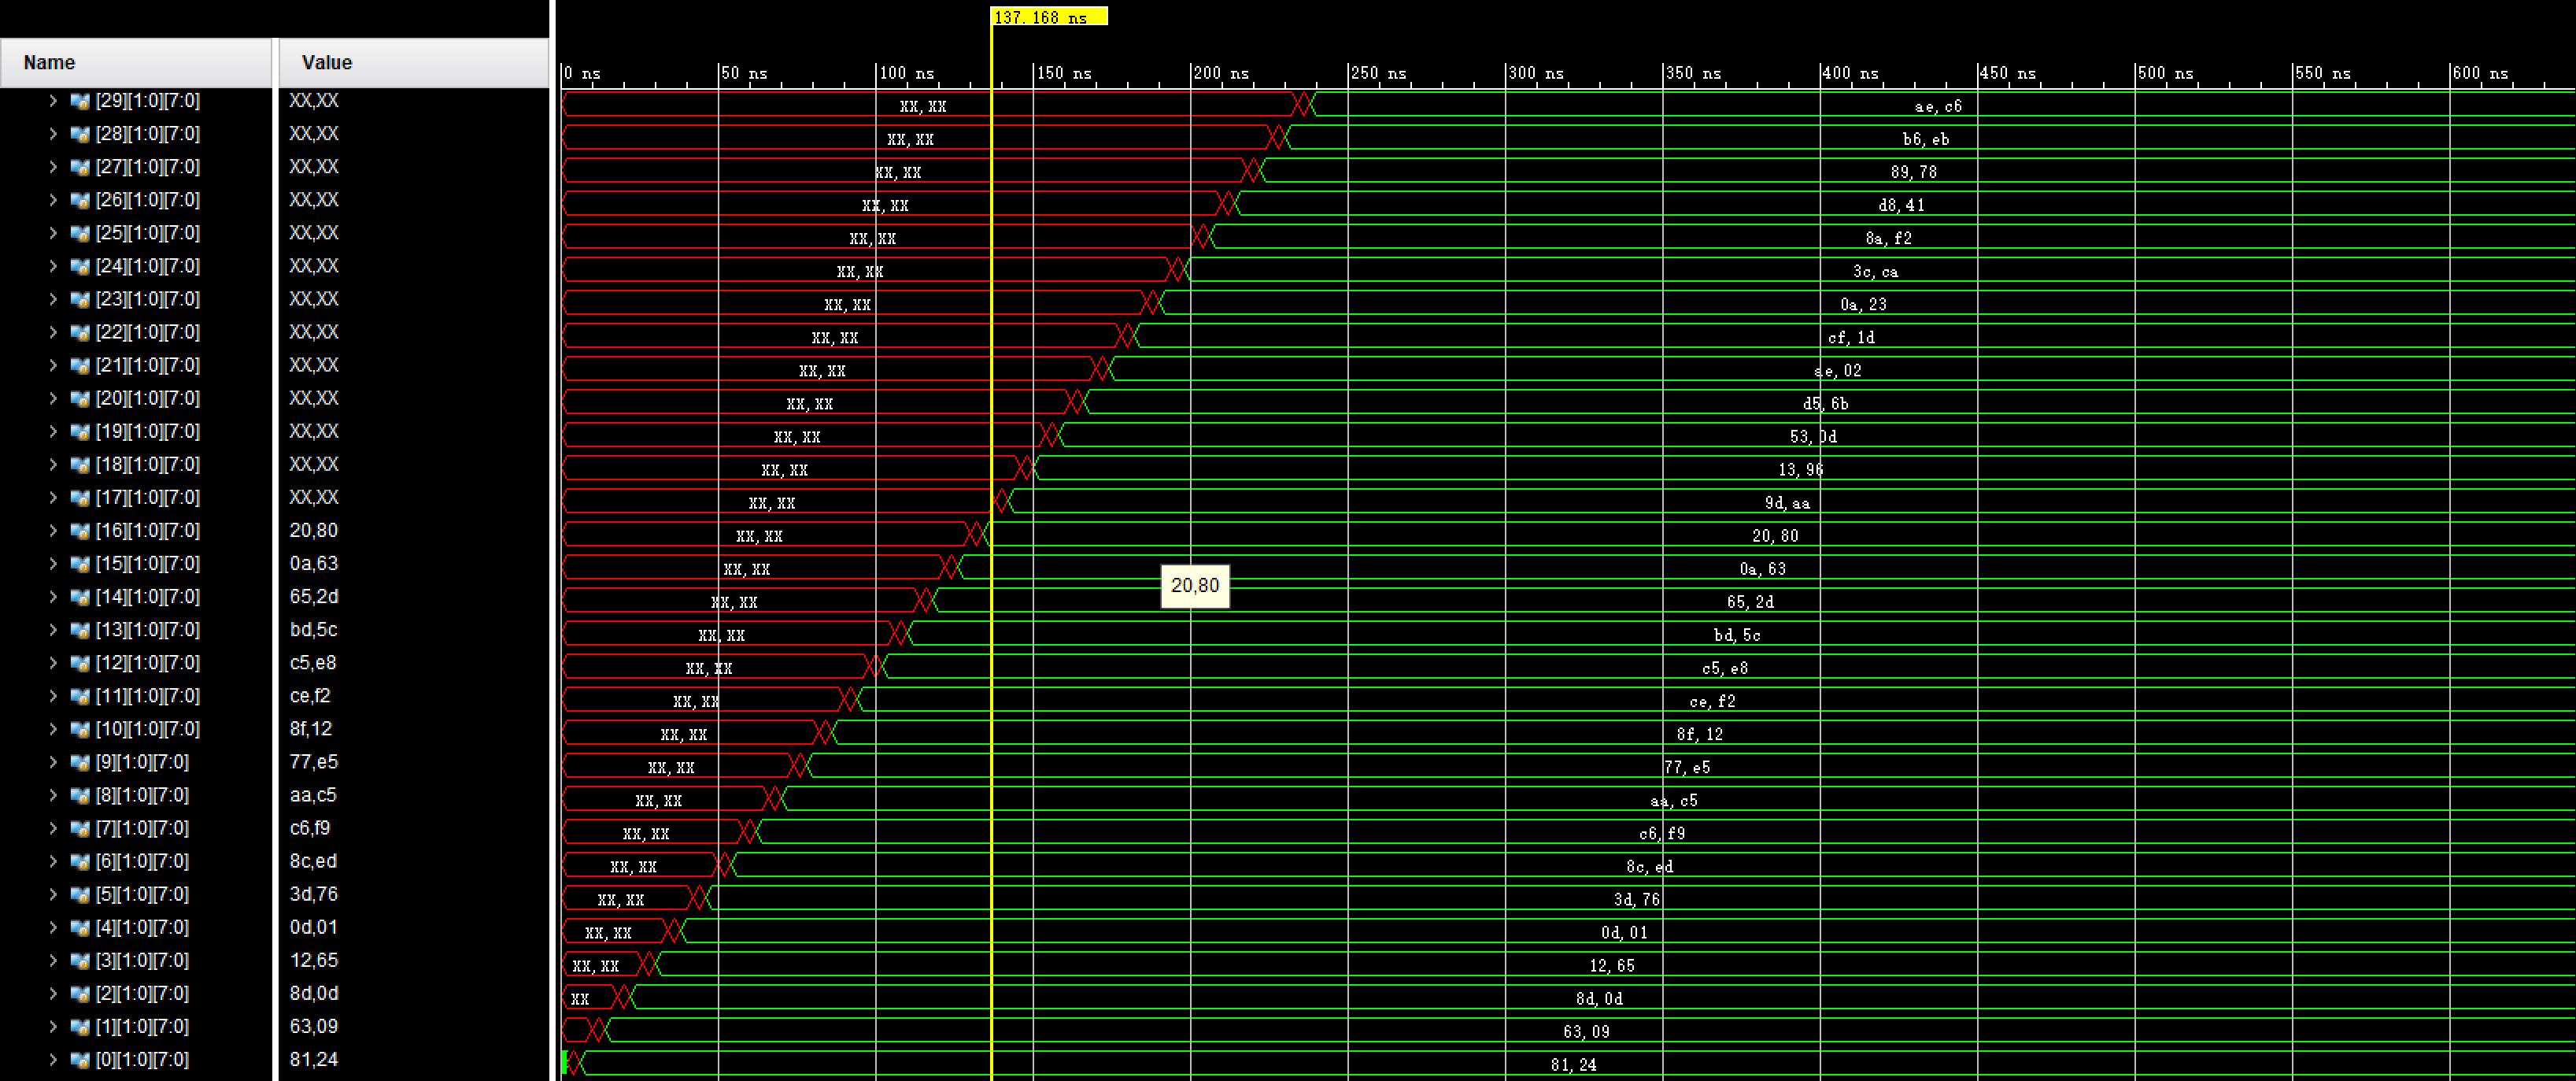
\includegraphics[width=\textwidth]{fifo_test_task1.png} % 需要替换成你的仿真图
    \caption{FIFO 模块的测试结果}
    \label{fig:fifo模块的测试结果}
\end{figure}

\section{实验二:实现循环读写FIFO}
\subsection{实验原理}
\subsubsection{FIFO 原理}
本次实验实现一个深度为 32,存储单元宽度为 16 bit 的 FIFO (First-In, First-Out) 缓冲器。FIFO 是一种先进先出的数据结构,数据按照写入的顺序被读取,常用于数据缓冲和速率匹配等场景。

\subsubsection{实现细节}
\begin{itemize}
    \item \textbf{数据存储:} 使用二维寄存器数组 \texttt{mem[31:0][1:0]} 来存储 FIFO 中的数据,每个存储位置可以存储两个 8 bit 数据,从而实现存储 16 bit 数据。
    \item \textbf{写入控制:} 通过 \texttt{input\_valid} 信号指示是否有新数据写入。 \texttt{input\_enable} 信号控制是否允许写入,当 FIFO 接近满时,\texttt{input\_enable} 置低,禁止写入。 \texttt{write\_addr} 作为写入地址指针。
    \item \textbf{读取控制:} 通过 \texttt{output\_enable} 信号控制是否允许读取。 \texttt{output\_valid} 信号指示 FIFO 是否有数据可读。当 FIFO 为空时, \texttt{output\_valid} 置低,禁止读取。\texttt{read\_addr} 作为读取地址指针。
    \item \textbf{数据宽度:} FIFO 存储的数据宽度是 16 位,但是读取时以 8 位方式读取,需要进行两次读取操作才能读取到全部 16 位数据。
    \item \textbf{满/空判断:} 当写入地址追上读取地址时,FIFO 被认为满,禁止写入;当读取地址追上写入地址时,FIFO 被认为空,禁止读取。
    \item \textbf{读取操作状态机:} 通过 \texttt{read\_state} 状态机控制读取操作,先读取低 8 位,再读取高 8 位。
\end{itemize}

\subsection{接口定义}
\begin{itemize}
    \item 输入信号:
    \begin{itemize}
        \item \texttt{clk}:时钟信号。
        \item \texttt{rstn}:复位信号,低电平有效。
        \item \texttt{input\_valid}:输入数据有效信号。
        \item \texttt{output\_enable}:输出使能信号。
        \item \texttt{data[15:0]}:16 位输入数据。
    \end{itemize}
    \item 输出信号:
    \begin{itemize}
        \item \texttt{write\_addr[4:0]}:写入地址指针。
        \item \texttt{read\_addr[4:0]}:读取地址指针。
        \item \texttt{input\_enable}:输入使能信号,指示 FIFO 是否可以写入数据。
        \item \texttt{output\_valid}:输出数据有效信号,指示 FIFO 是否有数据可读。
        \item \texttt{out[7:0]}:8 位输出数据。
    \end{itemize}
\end{itemize}

\subsection{调试过程及结果}
\subsubsection{代码分析}
模块 \texttt{task2\_module} 实现了深度为 32 的 FIFO 缓存器。核心逻辑包括使用 \texttt{mem} 数组存储数据,使用 \texttt{write\_addr} 和 \texttt{read\_addr} 指针管理数据的写入和读取。使用 \texttt{input\_enable} 和 \texttt{output\_valid} 信号来控制数据的写入和读取。数据按 16bit 写入的,按 8bit 读取的,并且使用 \texttt{read\_state} 状态机控制读取顺序。

\subsubsection{仿真验证}
在仿真测试中,我们验证了 FIFO 在不同输入条件下的正确性。我们通过控制 \texttt{input\_valid}, \texttt{output\_enable}, 和 \texttt{data} 输入,观察 \texttt{write\_addr}, \texttt{read\_addr}, \texttt{input\_enable}, \texttt{output\_valid} 和 \texttt{out} 输出,验证了 FIFO 的数据写入和读取功能。仿真波形显示了 FIFO 的满/空标志以及写入和读取地址的正确变化,以及输出数据的有效性。仿真结果如下:

\begin{figure}[H]
    \centering
    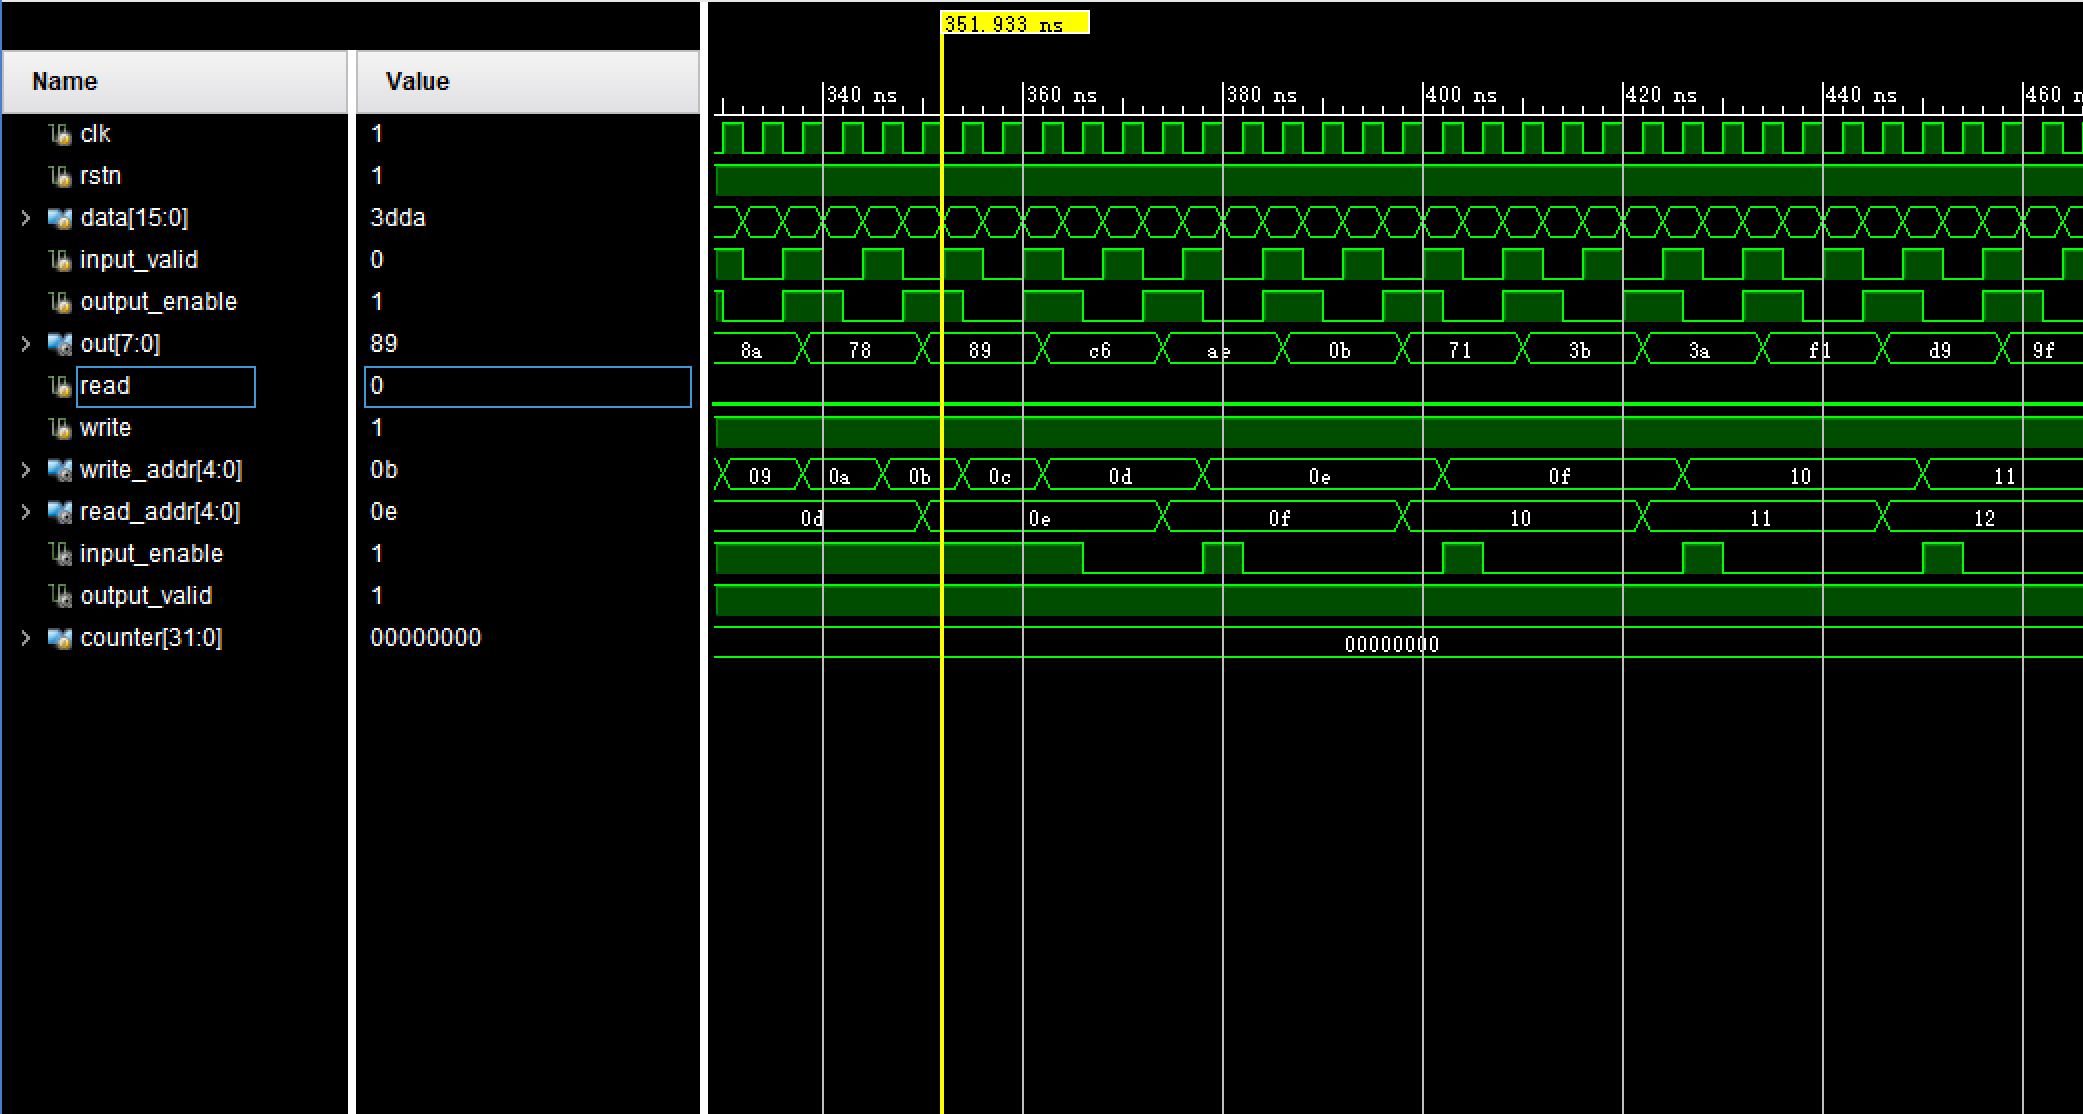
\includegraphics[width=\textwidth]{./exp_2_1_fifo.png} % 需要替换成你的仿真图
    \caption{FIFO 模块的测试结果}
    \label{fig:fifo模块的测试结果}
\end{figure}

根据上述波形图可以看出,当FIFO被写满时,只有向外读出一个数据时FIFO才能继续写入数据。可见这个FIFO模块的功能是正确的。

\begin{figure}[H]
    \centering
    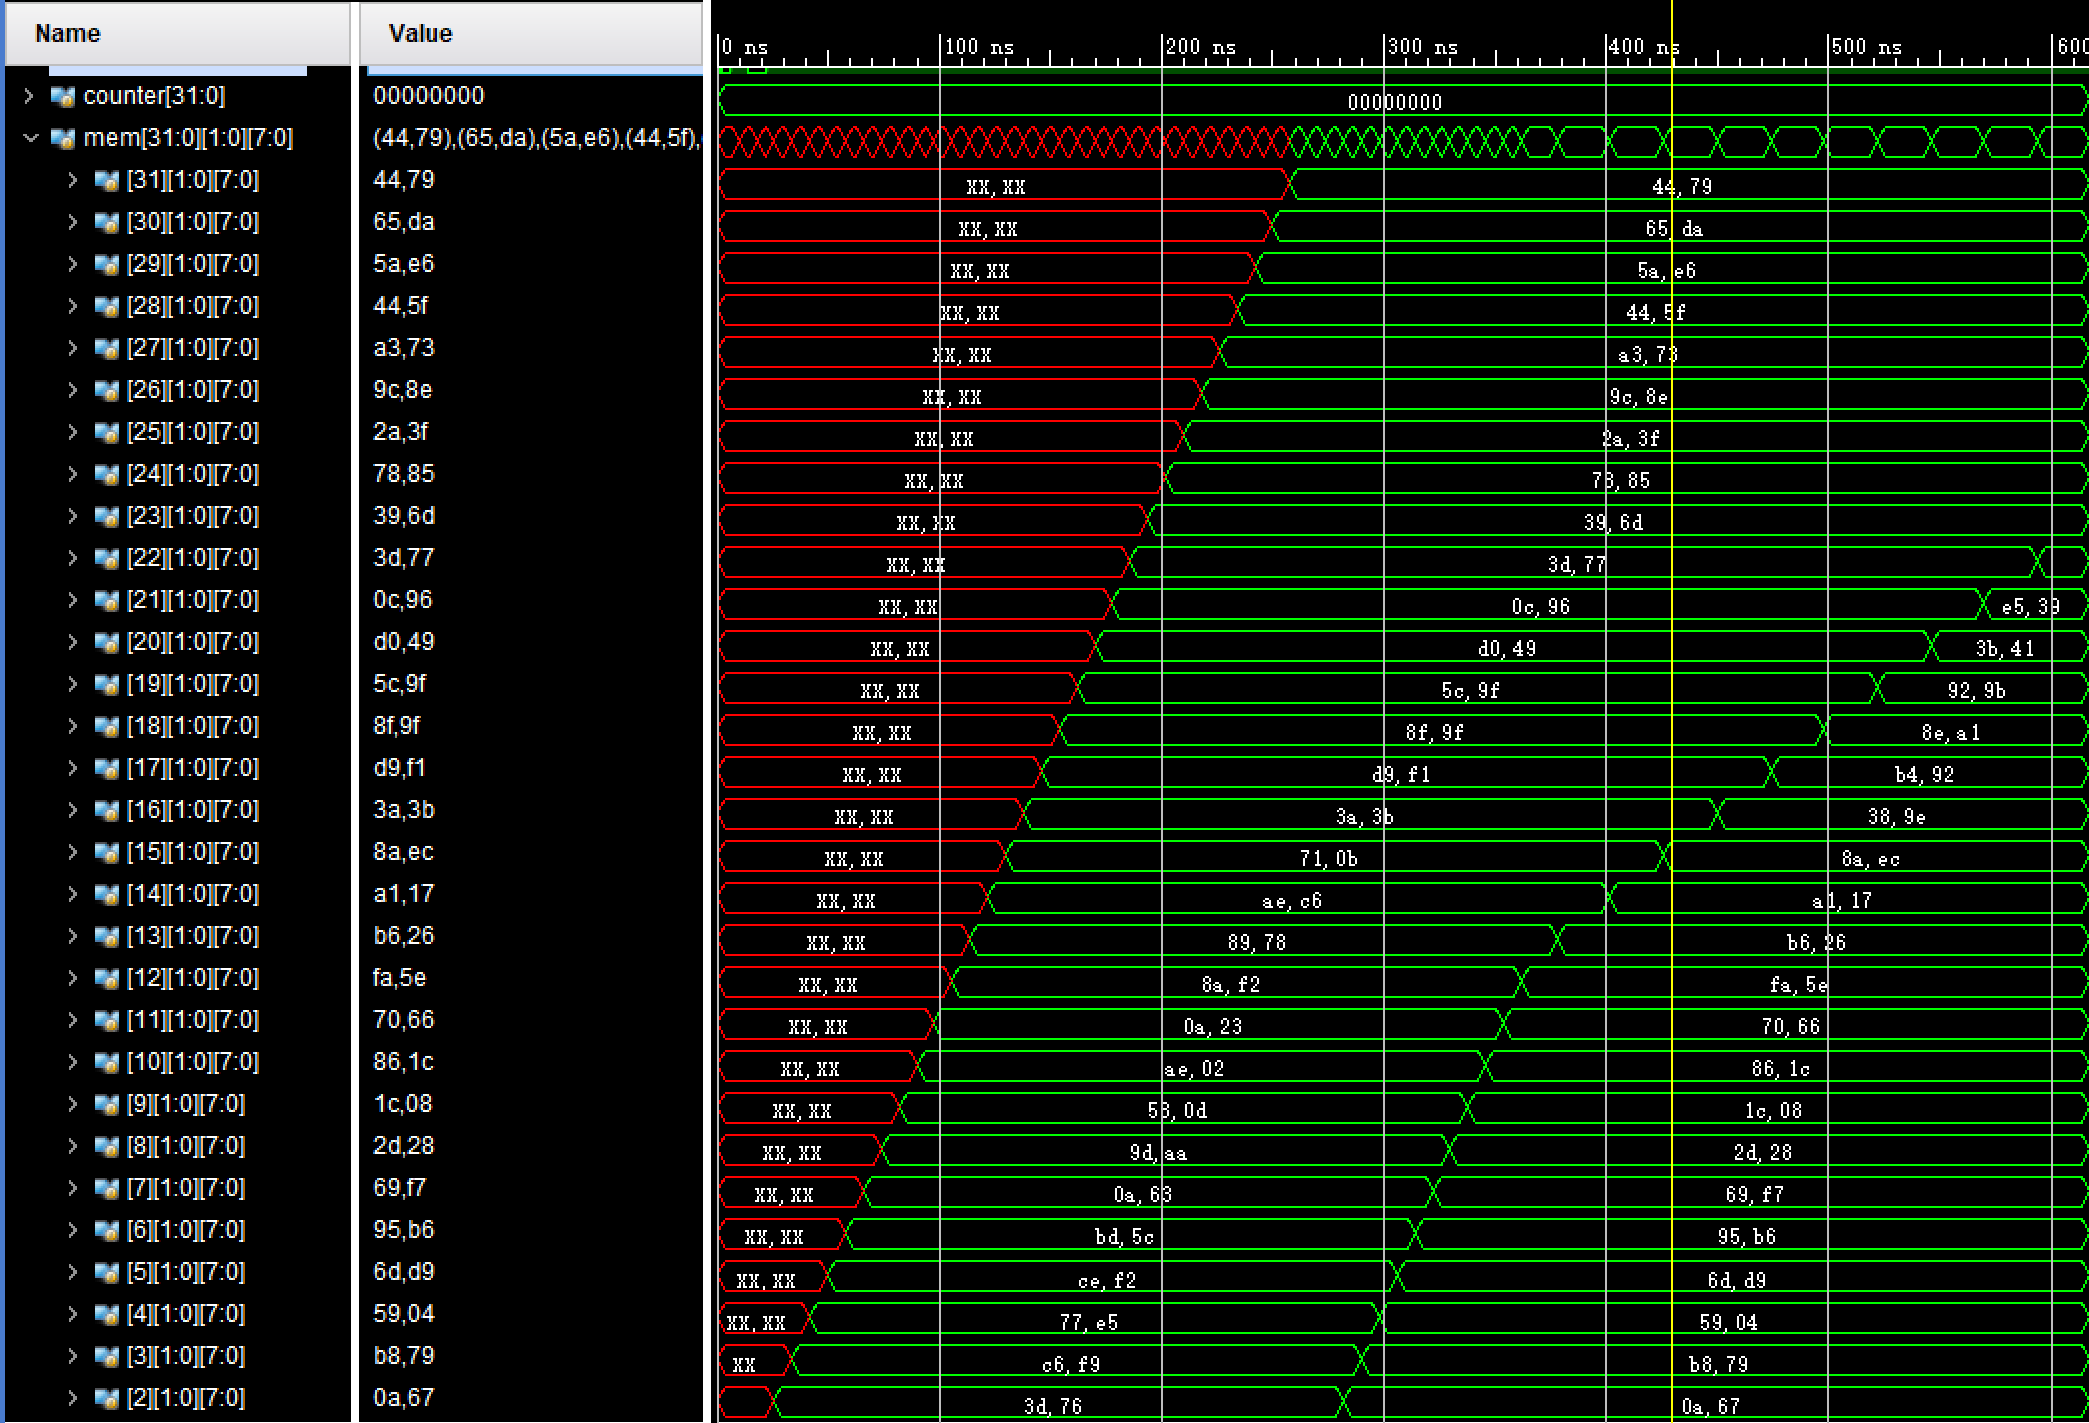
\includegraphics[width=\textwidth]{./cyclic_io.png} % 需要替换成你的仿真图
    \caption{FIFO模块的循环读写功能}
    \label{fig:fifo模块的循环读写功能}
\end{figure}

根据这个波形图可以看出,FIFO模块可以实现循环读写,在后边写入速度变慢的原因是因为由于在 testbench 中读出的频率比写入要慢,因此在后期 FIFO 处于写满状态,必须等待读出一个数据后方能写入下一个数据。

\section{实验三:实现FIFO的读写控制}

由于在实验二中实现的模块的读写位宽已经满足要求,因此在实验三中只需要实现读写控制即可。

\subsection{\texttt{task2\_module} 接口定义}

本次实验的模块仍然为为 \texttt{task2\_module},其接口定义如下:

\begin{itemize}
    \item \textbf{输入信号:}
    \begin{itemize}
        \item \texttt{clk}:时钟信号。
        \item \texttt{rstn}:复位信号,低电平有效。
        \item \texttt{input\_valid}:输入数据有效信号,指示输入数据 \texttt{data} 有效。
        \item \texttt{output\_enable}:输出使能信号,指示可以读取输出数据。
        \item \texttt{data [15:0]}:16位输入数据。
    \end{itemize}
    \item \textbf{输出信号:}
    \begin{itemize}
        \item \texttt{out [7:0]}:8位输出数据。
        \item \texttt{write\_addr [4:0]}:FIFO写地址。
        \item \texttt{read\_addr [4:0]}:FIFO读地址。
        \item \texttt{input\_enable}: FIFO可以写入信号。
        \item \texttt{output\_valid}:输出数据有效信号,指示输出数据 \texttt{out} 有效。
    \end{itemize}
\end{itemize}

\subsection{Testbench 描述}
Testbench 代码的主要功能如下:
\begin{itemize}
    \item \textbf{时钟和复位:} \texttt{clk} 生成一个周期为4个时间单位的时钟信号,\texttt{rstn} 生成一个复位信号,低电平有效。
    \item \textbf{输入信号:}
    \begin{itemize}
        \item \texttt{input\_valid} 信号以 8个时间单位的周期翻转,模拟输入数据的有效性。
        \item \texttt{output\_enable} 信号以 12个时间单位的周期翻转,模拟输出使能信号,由此,保证了读写频率之比为 3 : 2。
        \item \texttt{data} 信号随机生成16位的数据。
    \end{itemize}
    \item \textbf{仿真结束:} 仿真在600个时间单位后结束。
\end{itemize}

\subsection{仿真结果分析}
\begin{figure}[H]
    \centering
    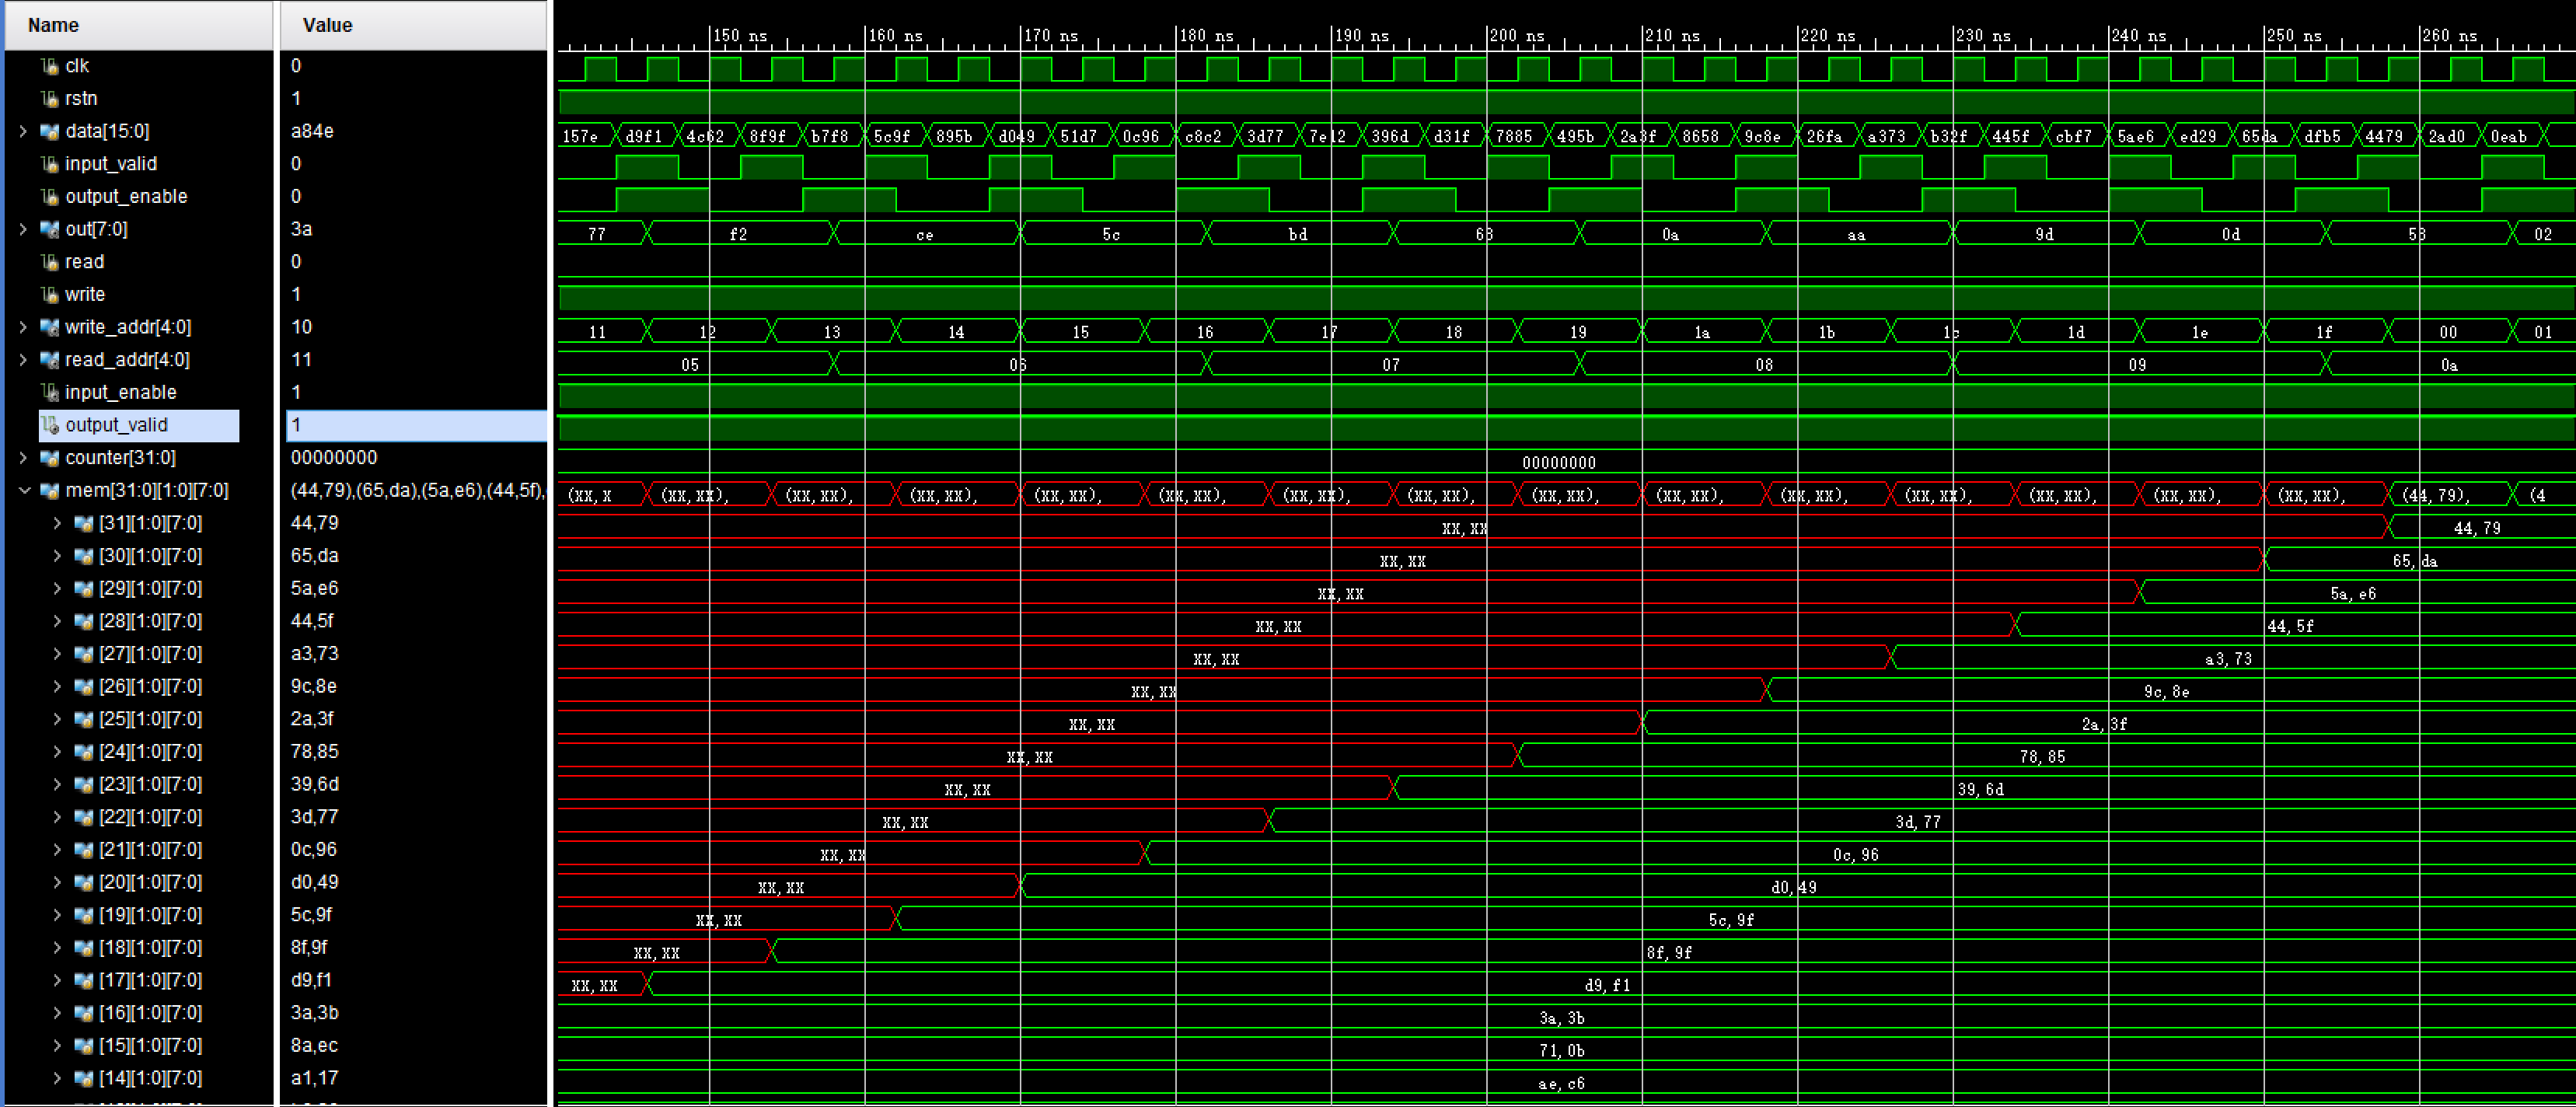
\includegraphics[width=\textwidth]{simulation_waveform.png} % 替换成你的波形图片路径
    \caption{\texttt{task2\_module} 模块的测试结果}
    \label{fig:task2_module模块的测试结果}
\end{figure}

根据上述波形图, \texttt{write\_addr} 和 \texttt{read\_addr}按照所希望的频率比变化。


\section{实验总结}

在本实验中,我通过 Verilog 实现了一个普通的同步FIFO模块,以及一个循环读写的FIFO模块。在实验过程中,我熟悉了FIFO的工作原理,以及如何通过状态机等方法实现FIFO的读写控制。在实验过程中,我通过仿真验证了FIFO的正确性。通过本次实验,我对FIFO的工作原理有了更深入的理解。

除此之外,在实现循环读写的FIFO模块的过程中,我实际上意识到了这是一个以双指针维护的环形队列。在实现过程中,我通过两个指针,一个指向写入位置,一个指向读取位置,来实现了循环读写的功能。这个过程中,我将程序设计课程中所学到的知识应用到了数字电路实验中,体会到了FIFO缓冲器与队列之间的联系。

\section{源代码}

\subsection{实验一:实现同步FIFO}

\begin{lstlisting}[language=Verilog]

module task1_module (
    input clk,
    input rstn,
    input input_valid,
    input output_enable,
    input [7:0] data,
    output reg [4:0] write_addr,
    output reg [4:0] read_addr,
    output reg input_enable,
    output reg output_valid,
    output reg [15:0] out
);

  reg fifo_empty;
  reg fifo_full;
  reg input_enable_next = 1'b1;

  reg [7:0] mem[31:0][1:0];

  reg [1:0] write_state;
  reg [1:0] read_state;

  always @(posedge clk) begin
    if (read_addr == 31) begin
      fifo_empty   = 1'b1;
      input_enable = 1'b1;
      output_valid = 1'b0;
    end else begin
      fifo_empty   = 1'b0;
      input_enable = 1'b0;
      output_valid = 1'b1;
    end
    if (write_addr == 31 && write_state == 2'b01) begin
      fifo_full = 1'b1;
      input_enable_next <= 1'b0;
      output_valid <= 1'b1;
    end else begin
      fifo_full = 1'b0;
      input_enable = 1'b1;
      output_valid = 1'b0;
    end
  end

  always begin
    #8;
    input_enable <= input_enable_next;
  end

  always @(posedge clk or negedge rstn) begin
    if (rstn == 0) begin
      write_addr <= 5'b0;
      read_addr <= 5'b0;
      write_state <= 2'b00;
      read_state <= 2'b00;
      fifo_empty <= 1'b1;
      fifo_full <= 1'b0;
      output_valid <= 1'b0;
      input_enable <= 1'b0;
    end else begin

      if (input_valid && input_enable) begin
        if (write_state == 2'b00) begin
          mem[write_addr][0] <= data;
          write_state <= 2'b01;
        end
        if (write_state == 2'b01) begin
          mem[write_addr][1] <= data;
          write_state <= 2'b00;
          write_addr <= write_addr + 1;
        end
      end

      if (output_valid && output_enable) begin
        out <= {mem[read_addr][1], mem[read_addr][0]};
        read_addr <= read_addr + 1;
      end
    end
  end
endmodule

\end{lstlisting}

实验一testbench代码如下:

\begin{lstlisting}[language=Verilog]

module task1_testbench ();

  reg clk, rstn;
  reg [7:0] data;
  reg input_valid, output_enable;
  wire [15:0] out;
  wire [4:0] write_addr, read_addr;
  wire input_enable, output_valid;

  task1_module task1_module_inst (
      .clk(clk),
      .rstn(rstn),
      .input_valid(input_valid),
      .output_enable(output_enable),
      .data(data),
      .out(out),
      .write_addr(write_addr),
      .read_addr(read_addr),
      .input_enable(input_enable),
      .output_valid(output_valid)
  );


  always #2 begin
    clk = ~clk;
  end

  initial begin
    clk  = 1'b0;
    rstn = 1'b1;
    #0.1 rstn = 1'b0;
    #0.2 rstn = 1'b1;
    input_valid = 1'b1;
  end

  always begin
    data = $random() % 9'b1_0000_0000;
    input_valid = 1'b1;
    output_enable = 1'b1;
    #4;
  end

  always begin
    #5;
    #6;
    #6;
    #360;
    rstn = 0;
    #4;
    rstn = 0;
    #370;
    $finish;
  end
endmodule

\end{lstlisting}

\subsection{实验二:实现循环读写FIFO}
\begin{lstlisting}[language=Verilog]

module task2_module (
    input clk,
    input rstn,
    input input_valid,
    input output_enable,
    input [15:0] data,
    output reg [4:0] write_addr,
    output reg [4:0] read_addr,
    output reg input_enable,
    output reg output_valid,
    output reg [7:0] out
);

  integer counter = 0;
  reg [7:0] mem[31:0][1:0];

  reg [1:0] write_state;
  reg [1:0] read_state;

  always @(posedge clk) begin
    if ((write_addr + 1) % 32 == read_addr) begin
      input_enable = 1'b0;
    end else begin
      input_enable = 1'b1;
    end
    if (write_addr == (read_addr + 1) % 32) begin
      output_valid = 1'b0;
    end else begin
      output_valid = 1'b1;
    end
  end

  always @(posedge clk or negedge rstn) begin
    if (rstn == 0) begin
      write_addr <= 5'b0;
      read_addr <= 5'b0;
      write_state <= 2'b00;
      read_state <= 2'b00;
      output_valid <= 1'b0;
      input_enable <= 1'b0;
    end else begin

      if (input_valid && input_enable) begin
        mem[write_addr][1] <= data[15:8];
        mem[write_addr][0] <= data[7:0];
        write_addr <= (write_addr + 1) % 32;
      end

      if (output_valid && output_enable) begin
        if (read_state == 2'b00) begin
          out <= mem[read_addr][0];
          read_state <= 2'b01;
        end else if (read_state == 2'b01) begin
          out <= mem[read_addr][1];
          read_state <= 2'b00;
          read_addr <= (read_addr + 1) % 32;
        end
      end
    end
  end
endmodule
\end{lstlisting}

\subsection{实验三:控制FIFO读写频率}
\begin{lstlisting}[language=Verilog]

module task2_testbench ();

  reg clk, rstn;
  reg [15:0] data;
  reg input_valid, output_enable;
  wire [7:0] out;
  reg read, write;
  wire [4:0] write_addr, read_addr;
  wire input_enable, output_valid;

  task2_module task2_module_inst (
      .clk(clk),
      .rstn(rstn),
      .input_valid(input_valid),
      .output_enable(output_enable),
      .data(data),
      .out(out),
      .write_addr(write_addr),
      .read_addr(read_addr),
      .input_enable(input_enable),
      .output_valid(output_valid)
  );


  always #2 begin
    clk = ~clk;
  end

  integer counter = 0;
  initial begin
    clk = 1'b0;
    rstn = 1'b1;
    write = 1'b0;
    read = 1'b0;
    input_valid = 1'b0;
    output_enable = 1'b0;
    #1 rstn = 1'b0;
    #2 rstn = 1'b1;
    #5;
  end

  always begin
    input_valid = ~input_valid;
    #4;
  end

  always begin
    output_enable = ~output_enable;
    #6;
  end

  always begin
    #4;
    data[7:0]  = $random() % 9'b100000000;
    data[15:8] = $random() % 9'b100000000;
  end

  always begin
    #5;
    write = 1'b1;
    #6;
    write = 1'b0;
    read  = 1'b1;
    #6;
    write = 1'b1;
    read  = 1'b0;
    #600;
    $finish;
  end
endmodule

\end{lstlisting}

\end{document}

% VScode 常用快捷键:

% F2:                       变量重命名
% Ctrl + Enter:             行中换行
% Alt + up/down:            上下移行
% 鼠标中键 + 移动:           快速多光标
% Shift + Alt + up/down:    上下复制
% Ctrl + left/right:        左右跳单词
% Ctrl + Backspace/Delete:  左右删单词    
% Shift + Delete:           删除此行
% Ctrl + J:                 打开 VScode 下栏(输出栏)
% Ctrl + B:                 打开 VScode 左栏(目录栏)
% Ctrl + `:                 打开 VScode 终端栏
% Ctrl + 0:                 定位文件
% Ctrl + Tab:               切换已打开的文件(切标签)
% Ctrl + Shift + P:         打开全局命令(设置)

% Latex 常用快捷键:

% Ctrl + Alt + J:           由代码定位到PDF


